\documentclass[letterpaper,oneside,openany,11pt]{book}
\usepackage[spanish]{babel} 
\usepackage[utf8]{inputenc}
\usepackage[authoryear, round]{natbib}
\usepackage{graphicx} % graficos
\usepackage{subfigure} % subfiguras
\usepackage[subfigure]{tocloft}
\usepackage{wrapfig}
\usepackage{enumerate} % enumerados
\usepackage{multirow} % para las tablas
\usepackage{longtable} % para tablas largas
\usepackage{lscape}
\usepackage{array}
\usepackage{titlesec}
\usepackage{tocloft}
\usepackage{longtable} % para tablas largas
\usepackage{amssymb, amsmath, amsbsy} % simbolitos
\usepackage{upgreek} % para poner letras griegas sin cursiva
\usepackage{cancel} % para tachar
\usepackage{mathdots} % para el comando \iddots
\usepackage{mathrsfs} % para formato de letra
\usepackage{stackrel} % para el comando \stackbin
\usepackage{amssymb}
\usepackage{float}
\usepackage{enumerate} 
\usepackage{caption}
\usepackage{lscape}
\DeclareCaptionLabelSeparator{point}{. }
\floatstyle{plaintop}
\restylefloat{table}

% para contraer referencias

\setlength{\textwidth}{155mm}
\setlength{\textheight}{215mm}
\setlength{\oddsidemargin}{6mm}
\setlength{\evensidemargin}{28mm}
\setlength{\topmargin}{-5mm}

{\setlength\tabcolsep{3.5pt} % default value: 6pt

\titleformat{\chapter}[hang]
{\vspace{-2.3cm}
	\normalfont\bfseries\huge}{\ \thechapter .}{0.0ex}
{
}
[
]

\captionsetup{
	position=above,
	justification=centering,
	labelsep=point, % <<< label and text on different lines
	singlelinecheck=false % <<< raggadright also when the caption is shorter
	% than a single line
}


\begin{document}
	
	\addtocontents{toc}{\hfill \textbf{Página} \par}
	\addtocontents{toc}{\vspace{-2mm} \hspace{-7.5mm} \hrule \par}
	
	% renombrar el Indice de cuadros por indice de tablas
	\renewcommand{\listtablename}{Índice de tablas}
	%renombrar cuadro por tabla
	\renewcommand{\tablename}{Tabla}
	\renewcommand{\cftfigfont}{Figura }
	\renewcommand{\cfttabfont}{Tabla }
	\renewcommand{\bibname}{Referencias}
	
\begin{titlepage}

% Empieza la portada 	
	\begin{center}
		\vspace*{-1in}
		\begin{figure}[htb]
			\begin{minipage}[b]{0.3\textwidth}
				\begin{center}
					
				\end{center}
				\end{minipage} \hfill \begin{minipage}[b]{0.6\textwidth}
				\scriptsize\textit{\begin{flushright}
						Tecnológico Nacional de México\\
						Instituto Tecnológico de Cd. Altamirano
					\end{flushright}}
		\end{minipage}
	\end{figure}
		

		\rule{160mm}{0.5mm}\\
		\vspace*{0.40in}
		\huge
		\textbf{Instituto Tecnológico de Cd. Altamirano}\\
		\vspace*{0.7in}
		
		\begin{large}
			\textbf{Informe técnico 2}\\
		\end{large}
		\vspace*{0.3in}
		\begin{Large}
			\textbf{Implementación de la metodología XP en un sistema tutor} \\
		\end{Large}
		\vspace*{0.4in}
		\begin{large}
			Presentan: \\
			\vspace*{0.25in}
			\textbf{Araujo Luviano Luis Fernando} \\
			\textbf{16930198} \\
		\end{large}
		\vspace*{0.4in}
		
		\begin{large}
			como requisito para la acreditación de la materia: \\
			\vspace*{0.1in}
			\textbf{Taller de Investigación II} \\
		\end{large}
		\vspace*{0.4in}
		
		\begin{large}
			Director de proyecto \\
			\vspace*{0.1in}
			\textbf{M.C. Leonel González Vidales} \\
		\end{large}
		\vspace*{0.4in}
	
		
		\vspace*{0.25in}
		\small
		Cd. Altamirano, Guerrero, México. \hfill Junio de 2020\\
		
	\end{center}
	
\end{titlepage}

% Pagina en blanco
\newpage
$\ $
\thispagestyle{empty} % para que no se numere esta pagina

% capitulo de dedicatorias
\chapter*{}
% \pagenumbering{Roman} % para comenzar la numeracion de paginas en numeros romanos

\begin{flushright}
 	\textit{Dedicado a \\
		mi familia}
 \end{flushright}
\thispagestyle{empty} % para que no se numere esta pagina
 
% Pagina en blanco
\newpage
$\ $
\thispagestyle{empty} % para que no se numere esta pagina

% Capitulo de agradecimientos 
\chapter*{Agradecimientos} % si no queremos que añada la palabra "Capitulo" 
\noindent Se le agradece al profesor M.C Leonel González Vidales por proporcionarme fuentes de información para completar las investigaciones y poder titularme.\\

Y un gran agradecimiento a mi familia por brindarme esta oportunidad de aprender en la materia de ingeniería en informática gracias a sus esfuerzos y tiempo para que yo pueda lograr titularme por sin sus sacrificios no estaría aquí y ahora.\\
\thispagestyle{empty} % para que no se numere esta pagina

% Pagina en blanco
\newpage
$\ $
\thispagestyle{empty} % para que no se numere esta pagina

\chapter*{Resumen} % si no queremos que añada la palabra "Capitulo"
\pagenumbering{arabic} % para empezar la numeración con números
\addcontentsline{toc}{chapter}{Resumen} % si queremos que aparezca en el índice
\markboth{Resumen}{Resumen} % encabezado
\noindent El XP es una metodología ágil para facilitar la elaboración de software en un tiempo determinado donde puede ser monitoreado por el cliente, con la finalidad de crear un software rápido y con el menor error posible y con una calidad excepcional, la metodología XP es una serie de paso a seguir para tener un óptimo desempeño.\\

El principal problema de esta metodología es que no se conoce muy bien en el ámbito estudiantil pasan por alto lo que significa y donde aplicarlo, así como otra metodología agiles como son las de scrum, RUP, Kanban, Agile inception y design sprint cada uno de ellos pertenece a las metodologías agiles, y cada una de ellas son diferentes entre si una mejores que otras, pero eso dependerá del tipo de proyecto que se desee realizar en instituciones u otros lugares donde manejen la informática, cada uno de ellos tienen sus ventajas y desventajas, pero se centrara en el uso de la metodología XP y los paso que tienen para terminar un proyecto de forma rápida.\\

Para que los alumnos conozcan este tipo de metodología se explicara los usos que se le pueden dar tanto en el ámbito laboral o personal ya sea para la creación de grandes proyectos escolares o empresariales, esta metodología tiene una serie de pasos parala elaboración del software y cada paso de la misma puede ser supervisada por el cliente para correcciones o modificaciones que se vallan ocurriendo al cliente en el transcurso del proyecto.\\

\chapter*{Abstract} % si no queremos que añada la palabra "Capitulo"
\addcontentsline{toc}{chapter}{Abstract} % si queremos que aparezca en el índice
\markboth{Abstract}{Abstract} % encabezado
\noindent XP is an agile methodology to facilitate the development of software in a given time where it can be monitored by the customer, in order to create a fast software with the least possible error and exceptional quality, the XP methodology is a series of steps to follow to have optimal performance.\\

The main problem of this methodology is that it is not well known in the student environment ignore what it means and where to apply it, as well as other agile methodology such as scrum, RUP, Kanban, Agile inception and design sprint each of them belongs to the agile methodologies, and each one of them are different from each other one better than others, but that will depend on the type of project you want to do in institutions or other places where they handle the computer, each of them have their advantages and disadvantages, but will focus on the use of XP methodology and the steps they have to finish a project quickly.\\

For students to know this type of methodology will explain the uses that can be given both in the workplace or personal either for the creation of large school or business projects, this methodology has a series of steps for the development of software and each step of it can be monitored by the client for corrections or modifications that occur to the client in the course of the project.\\

\newpage
\tableofcontents % indice de contenidos

\cleardoublepage
\addcontentsline{toc}{chapter}{Lista de figuras} % para que aparezca en el indice de contenidos
\listoffigures % indice de figuras

\cleardoublepage
\addcontentsline{toc}{chapter}{Lista de tablas} % para que aparezca en el indice de contenidos
\listoftables % indice de tablas	

% Resumen de la propuesta de Tesis

% La introducción proporciona una descripción precisa, breve y suficiente de cada una de las partes del proyecto. Se explica de una manera sencilla y clara la justificación, métodos, procedimientos utilizados, resultados obtenidos y conclusiones. También se exponen los motivos por los cuales el residente desarrollo dicho proyecto y la forma en que abordo el tema o el problema. Pueden incluirse reconocimientos o agradecimientos a aquellas personas e instituciones que ayudaron de alguna forma a la realización del proyecto ya sea con dinero, uso de instalaciones, acceso a documentos, orientaciones, préstamo o donación de bibliografía, materiales o equipo, etc. 

\chapter{Introducción}\label{cap.introduccion}
\noindent  En las metodologías agiles son series de paso para desarrollar un proyecto de forma corta y con una buena calidad, una de estas metodologías agiles es la XP con esta metodología se puede acortar el tiempo de creación de un proyecto, dado en los tiempos actuales se requiere que un software sea terminado de forma rápida y con el mínimo de errores, la metodología XP es una serie de 4 pasos de avance y retorno una de las ventajas de esta metodología es que el usuario puede dar su opinión si el proyecto cumple con sus expectativas o si requiere una modificación para que el software cumpla con las ideas del cliente.\\


% La justificación es la fundamentación del proyecto, donde se plantea la razón por la cuál el trabajo realizado es importante y trascendente. Donde los resultados obtenidos dan solución a las exigencias o expectativas académicas, sociales, empresariales, tecnológicas, científicas. Puede incluirse en detalle los antecedentes, causas e importancia de la situación que han motivado la realización del proyecto; asimismo, es conveniente comentar tanto los beneficios y ventajas que se derivan del proyecto, como sus desventajas y limitaciones. 

\chapter{Justificación}\label{cap.justificacion}
\noindent Al utilizar la metodología XP se pretender hacer un sistema tutor, en este caso al instituto tecnológico de ciudad Altamirano, con el fin de ayudar a los alumnos a desarrollar sus habilidades académicas o instruirlos en un tema específico.\\

Al ser una de las metodologías agiles podrá terminarse el proyecto de manera rápida y eficiente evitando errores de código, al hacerlo con esta metodología se pretende diseñar una pagina web para los alumnos de la institución, debido a los estándares bajos de los alumnos, que posiblemente tenga dificultad para aprender una o varias materias, claro esto es un hipo tesis.\\

Sin embargo, puede tener limitaciones en este caso de que falle la perdida de comisión pueden ser muy altas, pero su alcance puede ser para cualquier proyecto de corto pazo.\\



% Los objetivos constituyen el ..para qué.. del trabajo y se refieren a lo que se desea lograr con el proyecto de residencia, determinando metas concretas, debidamente cuantificables, éstos deben ser escritos de una manera precisa y clara. Cuando el objetivo del proyecto es muy general conviene dividirlo en objetivos específicos. 

% Según Rojas Soriano menciona que los objetivos son señalamientos provisionales que se contemplan y profundizan a medida que avanza el trabajo. 

\chapter{Objetivos}\label{cap.objetivos}

\section{Objetivo general}
\noindent Orientar el uso de la metodología XP ya que la escuela no cuenta con este tipo de orientación y sus usos y función, para posteriormente aplicarlos en la elaboración de software de forma rápida y con una calidad óptima. \\

\section{Objetivos espec\'{\i}ficos}
\begin{itemize}
\item Identificar concretamente que es la metodolog\'{\i}a XP y como utilizarlo para elaboración de un software.

\item Mostrar y a facilitar la creación de software de forma rápida y con una calidad alta.

\item Dar un software de calidad de forma rápida con el menor error posible.

\item Explicar las funciones que tiene la metodología XP y como esto tiene que ver con la creación de un software.

\end{itemize}


% Primeramente, se hace necesario entender lo que es un problema. Por lo tanto, la identificación de una necesidad o problema (dificultad a resolver) corresponde al análisis y evaluación de discrepancias mensurables entre una situación actual (lo que es) y otra deseada o necesaria (lo que debe ser, o debería ser) de un departamento, proceso o manejo de un sistema de información, etc. en una empresa u organismo. Donde este problema identificado se le dará solución al realizar el proyecto de residencia. Es posible que al realizar el análisis entre la situación actual y deseada surjan varios problemas a resolver; si esto sucede hay que priorizarlos. 

% La forma de plantear el problema es describir las discrepancias mensurables entre la situación actual y deseada sin poner las soluciones ni métodos o procedimientos para hacer algo. 

% Ejemplo: En los últimos tres años el porcentaje de alumnos reprobados en la materia xxxx siempre ha sido entre un 50 y 60 por ciento, ocupando el más alto índice de reprobados de todas las materias de la especialidad. La Comité Académico solicita a la Academia de la especialidad plantear alternativas de solución para que el porcentaje de reprobados no sobrepase del 5 por ciento para el próximo semestre. 

% NOTA: Hay que tener cuidado, por que no es raro que algunas personas protesten diciendo -ya sabemos cuáles son nuestros problemas, lo que necesitamos son soluciones-. Pero muchas veces sólo conocemos algunos síntomas de ciertos problemas; sin embargo, a menudo no tenemos conocimiento de la naturaleza exacta de cada problema o necesidad, dando como resultado a no resolver nunca el problema verdadero. Un caso análogo sería un médico que recetara una aspirina a un paciente con dolor de cabeza, para descubrir más tarde que el enfermo tenía un tumor cerebral. 


\chapter{Problemas a resolver}\label{cap.problemasresolver}
\noindent En la actualidad los alumnos tienen problemas para entender las materias impartidas por un profesor, debido que no tienen un modo diferente de aprender las cosas pueden entender por medio de lectura, visual o auditivo entre otras maneras, este a llevado a que los alumnos reprueben dicha materia, y no otra forma en que el alumno aprenda de otra manera, a no ser que se plante una alternativa para solucionar el número de reprobados. \\

Al resolver como los alumnos puedan aprender las materias de forma fácil lo siguiente de que manera lo harán y con metodología lo harán debe ser una fácil y Rápido de hacer con los errores menores, para evitar que los alumnos sigan reprobando las materias a la más brevedad posible.\\


% Es la exposición organizada de los elementos teóricos generales y particulares (metodologías, procesos, otros trabajos. o Tesis planteadas por investigadores reconocidos.

% Ejemplo: algunos principios de la Ingeniería de Software o de la Administración), así como la explicitación de los conceptos básicos en que se apoya tu proyecto de residencia. Se puede decir que ese fundamento teórico y conceptual representa la posición teórica del residente como base en la cual plantea el problema y centra la búsqueda de soluciones a las necesidades (problemas) planteadas. 

% Para redactar el fundamento teórico es suficiente que el residente: 

% Escriba el nombre de la teoría sustentada o en su defecto el nombre del autor o autores más importantes en los cuales se basó para abordar el problema que dio lugar al desarrollo de su trabajo. 
% Explique o describa la teoría en cuestión o las tesis sostenidas por el autor. 
% Defina o explique los conceptos o principios que son propios de la teoría en cuestión o de las tesis planteadas por investigadores. 
% Indique la o las fuentes en las que se documentó para elaborar este fundamento teórico que guió el abordaje del proyecto. 

\chapter{Fundamento  teórico}\label{cap.marco}

\noindent  Según \cite{Thiyagarajan} y \cite{Com} el \textit{extreme programming}(XP) es una de las metodología agiles para el desarrollo de software de mayor exito y controversiales que existen en los tiempos actuales. \\

esto quiere decir que permite a los usuarios tener un software fiable y funcional rápidamente y continuar con un desarrollo a un ritmo rápido de forma segura y predecible con una calidad cada vez mayor con un diseño para poder adaptarse a los entornos donde los requisitos están cambiando de forma rápida y cuyo alcance no está claro. esto con el fin de conseguir la satisfacción del cliente. \\

A continuación se mostrara el proceso de la metodología XP como se ve en la Figura 2.1.\\

\begin{figure}[H]
	\centering
	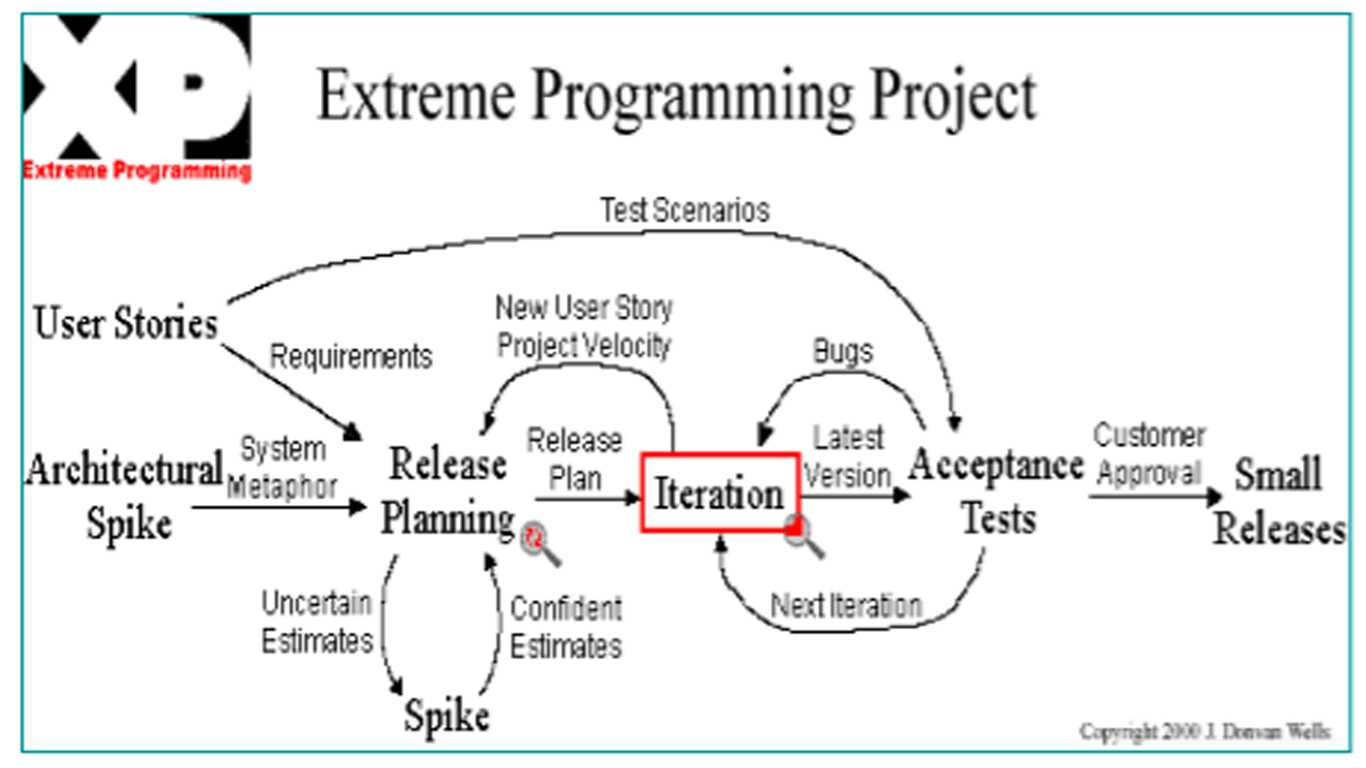
\includegraphics[width=1.0\textwidth]{./Imagenes/1}
	\caption{Proceso de la metodología XP.}
\end{figure}

 Según \cite {Com} Comenta que La metodología XP es una serie de pasos a seguir para elaboración de un proyecto ya sea para las instituciones o en otros lugares esto muy usado para elaboración de software a base de pruebas y error, y para lograr esto se centra principalmente en la interacción directa con los usuarios donde estos dan su opinión a lo largo de siclo de vida del proyecto.\\ 

\section{Metodología Scrum}
\noindent Según \cite{Com} como se dicta el scrum es una metodología que mantiene las cosas simples en un ambiente de negocios con un constate cambios esto quiere decir es que reuniones dirías y agotadoras por parte del equipo de proyecto con un único propósito de entregar un software de calidad en un periodo no menor de 24 horas lo que se denomina “sprints”. \\

A continuación se mostrara el proceso de la metodología Scrum como se ve en la Figura 2.2.\\

\begin{figure}[H]
	\centering
	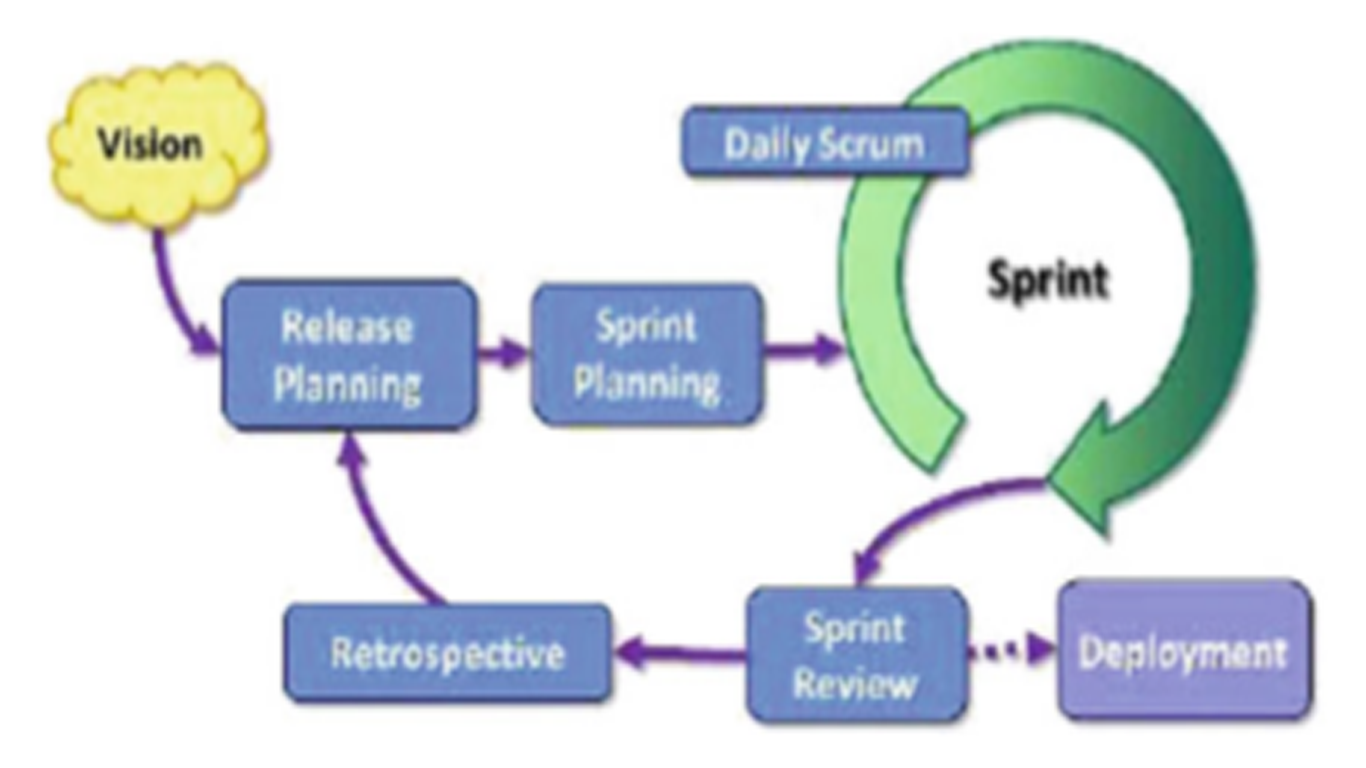
\includegraphics[width=1.0\textwidth]{./Imagenes/2}
	\caption{Proceso de la metodología Scrum flow.}
\end{figure}

\section{Metodología RUP}
\noindent Según \cite{Chacon} Por sus siglas en inglés \textit{Rational Unified Process}(Proceso Unificado de Rational) es una metodología que permite asignar tareas y responsabilidades dentro de una organización de desarrollo. Para producir software de alta calidad lo que permite resolver las necesidades de los usuarios dentro de propuestas y un tiempo establecido. \\

La RUP tiene dos dimensiones una con un eje vertical y la otra con un eje horizontal.\\

\begin{itemize}
	\item El eje horizontal: representa un tiempo y demuestra los aspectos de vida del proceso.
	
	\item El eje vertical: representa las diciplinas que agrupan actividades definidas lógicamente por la naturaleza.
\end{itemize}
La primera dimensión es representada con un proceso dinámico y se expresa en términos de fases, de iteraciones, y la finalización de las fases.
La segunda dimensión representa el aspecto estático: cómo son , las disciplinas, las actividades, los flujos de trabajo, los artefactos, y los roles. \\

En la Figura 2.3, se puede observar como varía el énfasis de cada disciplina en un cierto plazo en el tiempo, y durante cada una de las fases. \\

\begin{figure}[H]
	\centering
	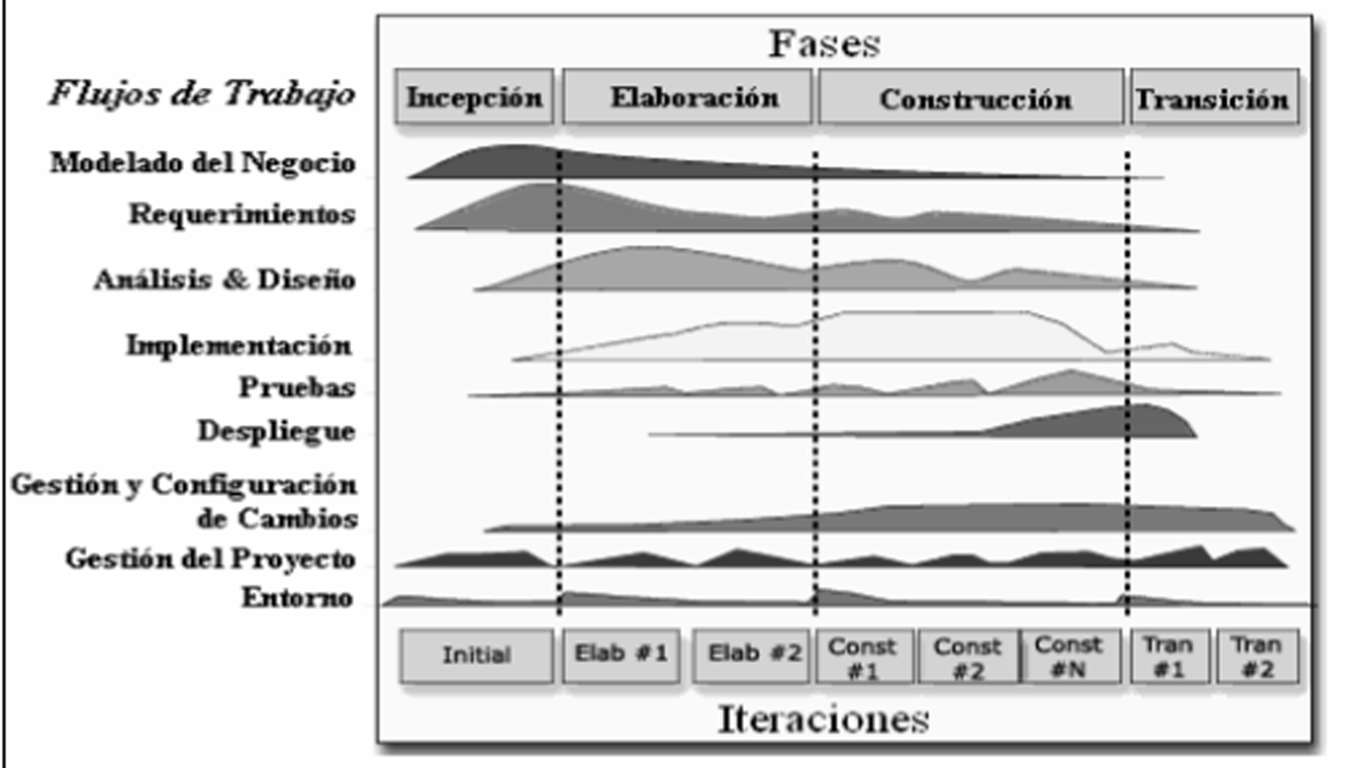
\includegraphics[width=1.0\textwidth]{./Imagenes/3}
	\caption{Disciplinas, fases, iteraciones del RUP.}
\end{figure}

\section{Metodología Kanban}
\noindent Según \cite{David} Kanban Es una herramienta que plantea los recursos de cuándo y cuanto trabajo se comprometen a hacer y los recursos toman el trabajo cuando están listo esto puede compararse a una impresora se envía a imprimir la maquina toma su tiempo para listo y entonces la página es expulsa del dispositivo.
\\
Kanban es una herramienta que permite trabajar más eficazmente que con la metodología scrum, es una herramienta muy adaptable hala hora de hacer un proyecto.\\

El Kanban tiene las siguientes características.
\begin{itemize}
	\item Elimina desperdicios.
	\item Determina el flujo de valor.
	\item Aumenta la velocidad al acortar el ciclo de tiempo.
\end{itemize}

\section{Metodología Agile Inception}
\noindent Según \cite{David} es una serie de dinámicas para que todo el personal se centre en un proyecto donde el objetivo es el mismo y así reduciendo muchas de las incertidumbres, y así ayudar a reducir los riesgos más evidentes.\\

Este tipo de metodología reúne a varios de las personas para iniciar un proyecto, pero muchas de los integrantes no pueden estar de acuerdo para esto es esto se basa en realización de preguntas y ejercicios que es de mucha utilidad antes de empezar un proyecto.
\\

En la Figura 2.4 se muestra cómo se pueden poner de acuerdo para creación de un proyecto.\\
\begin{figure}[H]
	\centering
	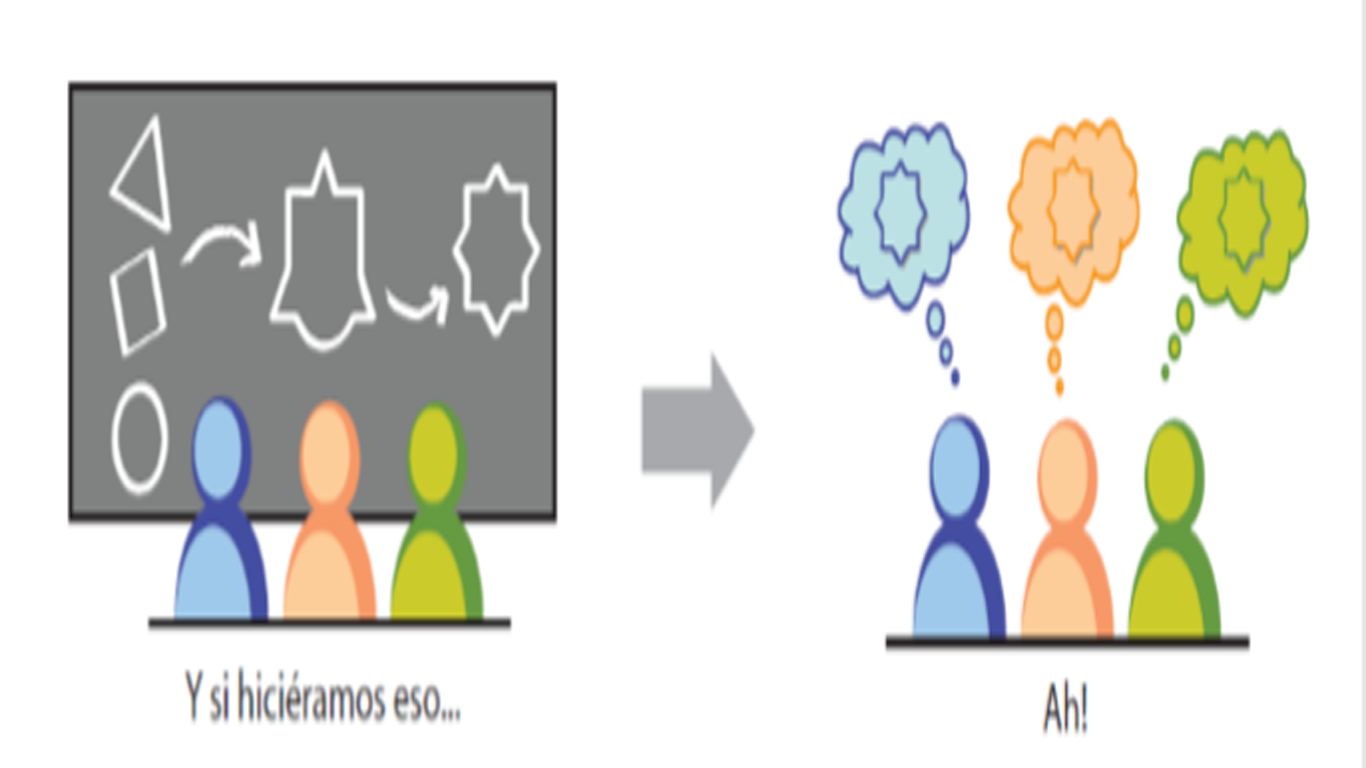
\includegraphics[width=1.0\textwidth]{./Imagenes/4}
	\caption{Solución en proyecto.}
\end{figure}

\section{Design Sprint}
\noindent Según \cite{App} es un marco para validar ideas a través de prototipos rápidos de las cuales Constantán de 5 fases.\\

Etapa 1: comprender: se evalúa el problema que se quiere resolver para que esta diseñado y en la forma en que se va utilizar.\\
Etapa 2: Divergencia: en esta se les alienta a que participen sin importar que tan loca sea la idea.\\
Etapa 3: Decidir: a través de una actividad los participan deciden cual es la idea a seguir.\\
Etapa 4: Prototipo: en esta etapa los participantes diseñan un prototipo de sus ideas para el proyecto.\\
Etapa 5: Validar: los participantes muestran su proyecto enfrente de los usuarios y si uno los anima solo se lo dicen.\\


% Esta sección debe contener las metodologías utilizadas y en general todos los procedimientos teóricos y prácticos que se hayan empleado. De hecho debe contemplar el qué se hizo, cómo se realizó, con qué equipo o material, cuándo, quiénes participaron y para qué se usaron tales procedimientos o métodos. 

% Si en el desarrollo del proyecto se utilizó equipo de cómputo, software o cualquier otro material, hay que incluir especificaciones técnicas, las cantidades, la procedencia. Si se realizaron procesos describir los métodos de preparación adjuntando tablas, gráficas, diagramas y figuras utilizadas. 

% Las actividades realizadas en una metodología deben presentarse en forma secuencial con un orden cronológico. 

% Si se realizan entrevista o encuestas es importante describir las características de la población estudiada, los controles utilizados en la selección de la muestra, tales como edad, sexo, escolaridad, nivel socioeconómico, tamaño de la muestra, etc. 

\chapter{Procedimiento y descripción de las actividades realizadas}\label{cap.procedimiento}
\section{Planificación}
\noindent El usuario nos proporcionara los datos necesarios para elaborar el programa, estos van desde las materias impartidos el número del alumno, además de las funciona que quiera que realice el programa y cuanto de estas funciones va tener.\\ 

Las siguientes funciones que el cliente desea son las siguientes:\\

\subsection{Fase De Análisis}
\noindent Se realizo un test de inteligencia a un determinado número de alumnos en el instituto tecnológico de ciudad Altamirano, en la carrera de ingenieros en informática. El test se hiso a los diferentes semestres de la carrera con el fin de conocer en tipo de inteligencia podría funcionar mejor con la mayoría de alumnos de la carrera, con el fin de evitar el número de reprobados.\\

\begin{figure}[H]
	\centering
	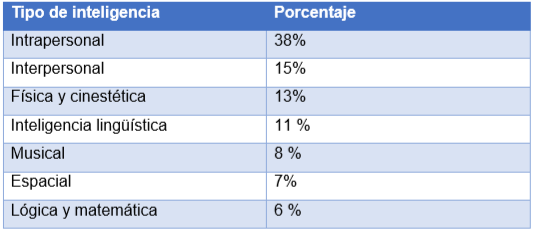
\includegraphics[width=1.0\textwidth]{./Imagenes/8}
	\caption{Se muestra el porcentaje de los alumnos}
\end{figure}

\subsection{Propósito}
\noindent \\

\subsection{Alcances}
\noindent \\

\subsection{Declaración del problema}
\noindent \\

\begin{figure}[H]
	\centering
	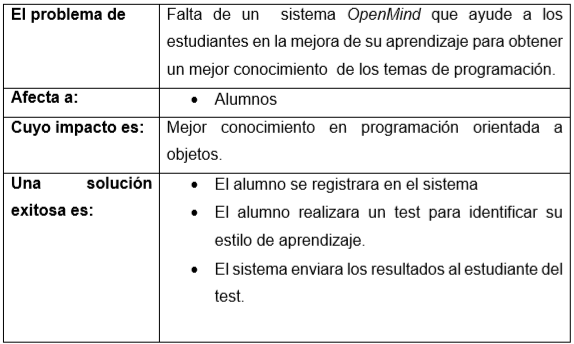
\includegraphics[width=1.0\textwidth]{./Imagenes/9}
	\caption{Se muestra el porcentaje de los alumnos}
\end{figure}

\subsection{Declaración de posición del producto tabla 3}
\noindent \\

\begin{figure}[H]
	\centering
	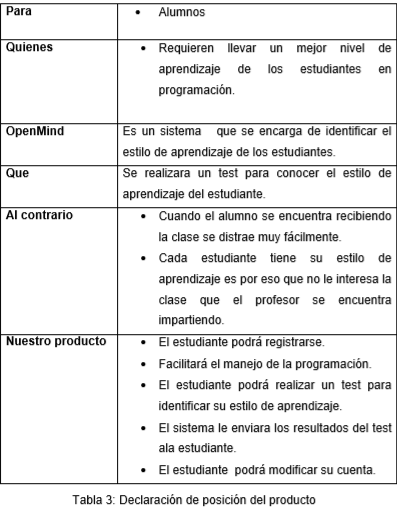
\includegraphics[width=1.0\textwidth]{./Imagenes/10}
	\caption{Se muestra el porcentaje de los alumnos}
\end{figure}

\subsection{Resumen de usuarios tabla 4}
\noindent \\

\begin{figure}[H]
	\centering
	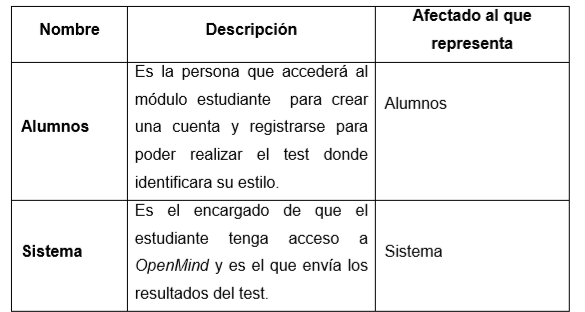
\includegraphics[width=1.0\textwidth]{./Imagenes/11}
	\caption{Se muestra el porcentaje de los alumnos}
\end{figure}

\subsection{Resumen del producto}
\noindent \\

\subsection{Funciones del sistema}
\noindent \\

\subsection{Supuestos y dependencias}
\noindent \\

\subsection{Diagrama de casos de uso}
\noindent \\

\begin{figure}[H]
	\centering
	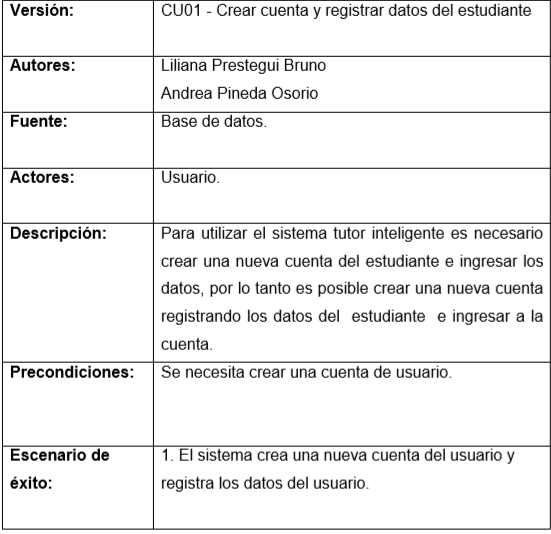
\includegraphics[width=1.0\textwidth]{./Imagenes/12}
	\caption{Se muestra el porcentaje de los alumnos}
\end{figure}

\begin{figure}[H]
	\centering
	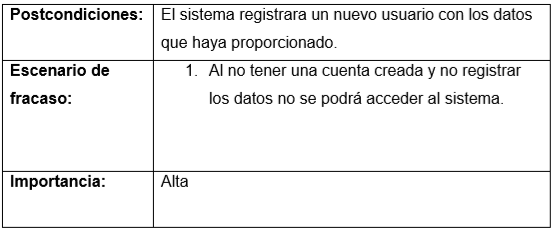
\includegraphics[width=1.0\textwidth]{./Imagenes/13}
	\caption{Se muestra el porcentaje de los alumnos}
\end{figure}

\begin{figure}[H]
	\centering
	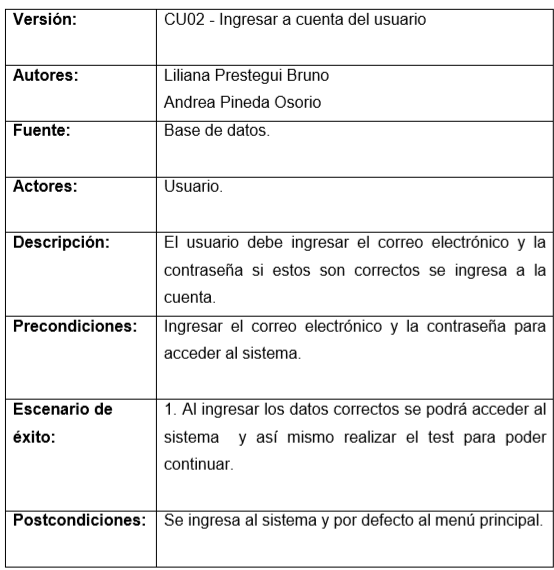
\includegraphics[width=1.0\textwidth]{./Imagenes/14}
	\caption{Se muestra el porcentaje de los alumnos}
\end{figure}

\begin{figure}[H]
	\centering
	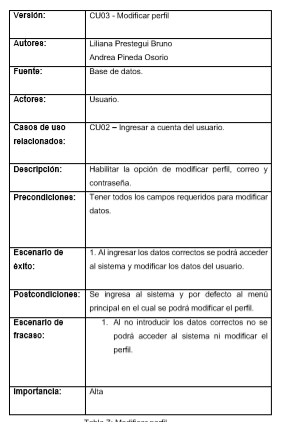
\includegraphics[width=1.0\textwidth]{./Imagenes/15}
	\caption{Se muestra el porcentaje de los alumnos}
\end{figure}

\begin{figure}[H]
	\centering
	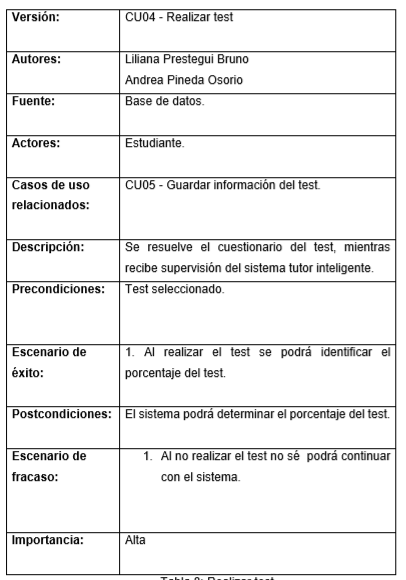
\includegraphics[width=1.0\textwidth]{./Imagenes/16}
	\caption{Se muestra el porcentaje de los alumnos}
\end{figure}

\begin{figure}[H]
	\centering
	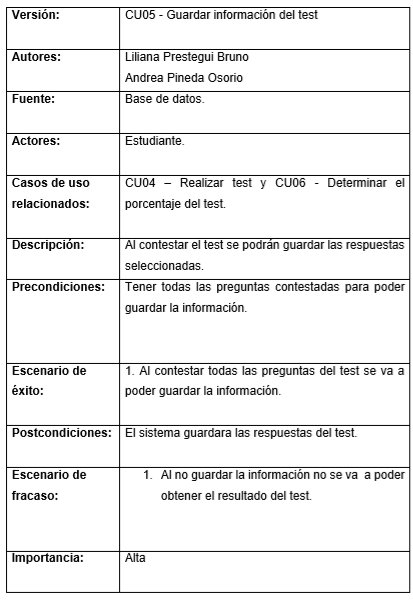
\includegraphics[width=1.0\textwidth]{./Imagenes/17}
	\caption{Se muestra el porcentaje de los alumnos}
\end{figure}

\begin{figure}[H]
	\centering
	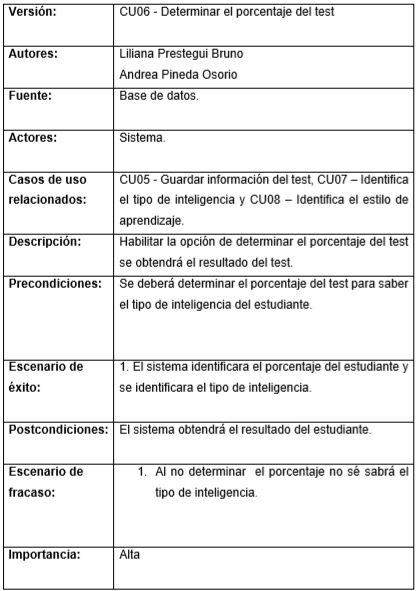
\includegraphics[width=1.0\textwidth]{./Imagenes/18}
	\caption{Se muestra el porcentaje de los alumnos}
\end{figure}

\begin{figure}[H]
	\centering
	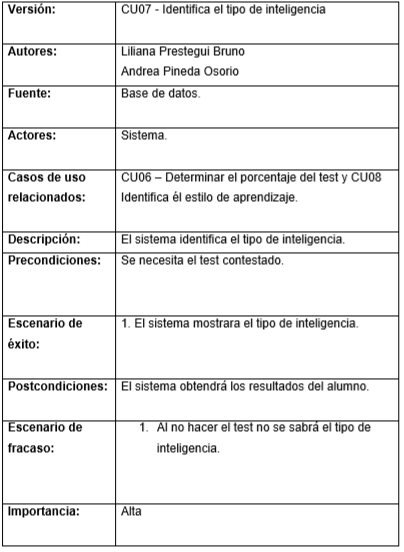
\includegraphics[width=1.0\textwidth]{./Imagenes/19}
	\caption{Se muestra el porcentaje de los alumnos}
\end{figure}

\begin{figure}[H]
	\centering
	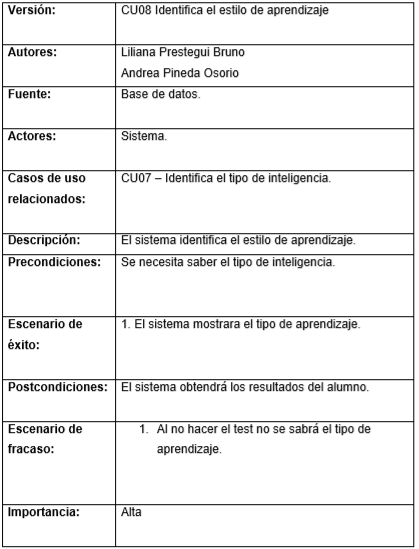
\includegraphics[width=1.0\textwidth]{./Imagenes/20}
	\caption{Se muestra el porcentaje de los alumnos}
\end{figure}

\begin{figure}[H]
	\centering
	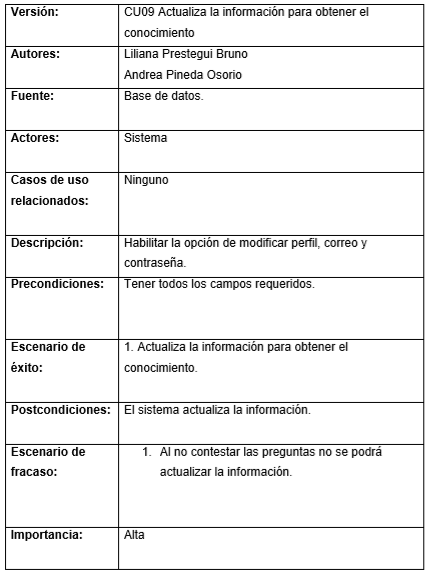
\includegraphics[width=1.0\textwidth]{./Imagenes/21}
	\caption{Se muestra el porcentaje de los alumnos}
\end{figure}

\begin{figure}[H]
	\centering
	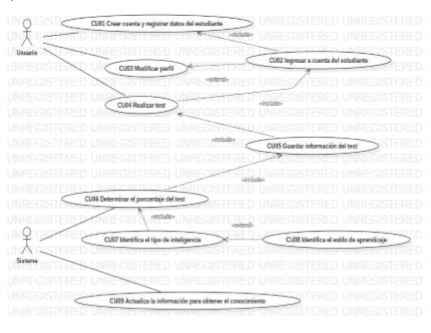
\includegraphics[width=1.0\textwidth]{./Imagenes/22}
	\caption{Se muestra el porcentaje de los alumnos}
\end{figure}

\begin{figure}[H]
	\centering
	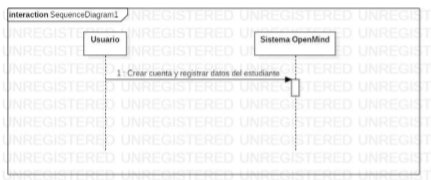
\includegraphics[width=1.0\textwidth]{./Imagenes/23}
	\caption{Se muestra el porcentaje de los alumnos}
\end{figure}

\begin{figure}[H]
	\centering
	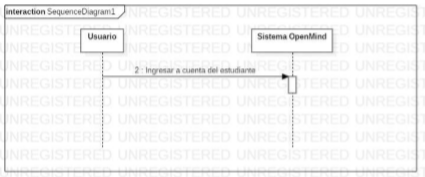
\includegraphics[width=1.0\textwidth]{./Imagenes/24}
	\caption{Se muestra el porcentaje de los alumnos}
\end{figure}

\begin{figure}[H]
	\centering
	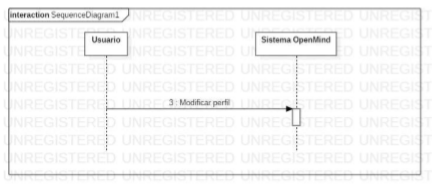
\includegraphics[width=1.0\textwidth]{./Imagenes/25}
	\caption{Se muestra el porcentaje de los alumnos}
\end{figure}

\begin{figure}[H]
	\centering
	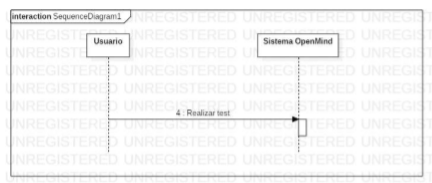
\includegraphics[width=1.0\textwidth]{./Imagenes/26}
	\caption{Se muestra el porcentaje de los alumnos}
\end{figure}

\begin{figure}[H]
	\centering
	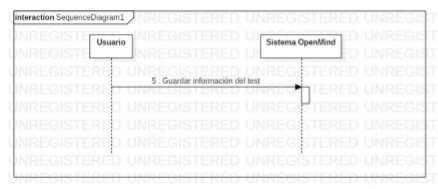
\includegraphics[width=1.0\textwidth]{./Imagenes/27}
	\caption{Se muestra el porcentaje de los alumnos}
\end{figure}

\begin{figure}[H]
	\centering
	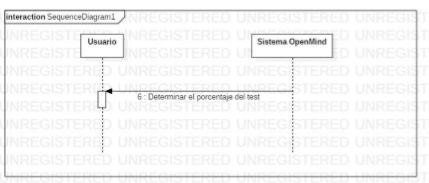
\includegraphics[width=1.0\textwidth]{./Imagenes/28}
	\caption{Se muestra el porcentaje de los alumnos}
\end{figure}

\begin{figure}[H]
	\centering
	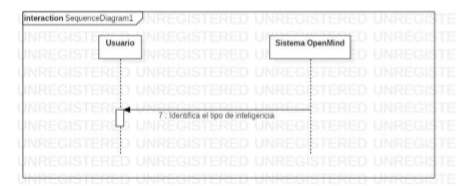
\includegraphics[width=1.0\textwidth]{./Imagenes/29}
	\caption{Se muestra el porcentaje de los alumnos}
\end{figure}

\begin{figure}[H]
	\centering
	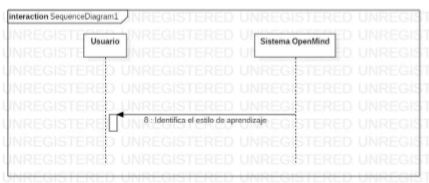
\includegraphics[width=1.0\textwidth]{./Imagenes/30}
	\caption{Se muestra el porcentaje de los alumnos}
\end{figure}

\begin{figure}[H]
	\centering
	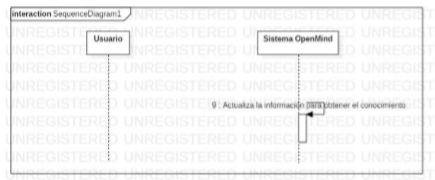
\includegraphics[width=1.0\textwidth]{./Imagenes/31}
	\caption{Se muestra el porcentaje de los alumnos}
\end{figure}

\subsection{Diagrama de base de datos}
\noindent \\

\begin{figure}[H]
	\centering
	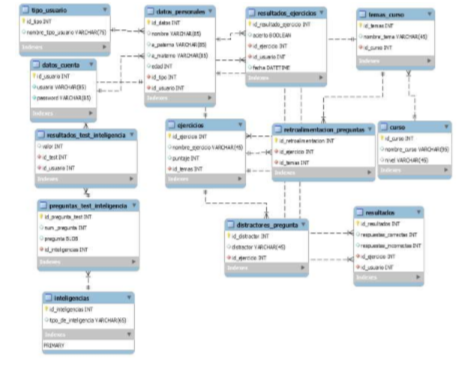
\includegraphics[width=1.0\textwidth]{./Imagenes/32}
	\caption{Se muestra el porcentaje de los alumnos}
\end{figure}

\section{Diseño}
\noindent Una ves proporcionado los datos dará inicio al diseño del programa, el usuario revisara si el diseño es de su agrado o requiere otra opción o una nueva función, esto puede variar desde el color del programa o qué hay muchas funciones o menos ya eso dependerá totalmente del usuario.\\
 
 \section{Codificación}
 \noindent Una ves creado el diseño y haya sido del agrado de usuario se habrá paso a la codificación generalmente es programado con dos personas para que den su punto de vista, en otras palabras, si un programador no logra ver el error el otro lo puede ayudar a encontrarlo o sugerir una solución obvia.\\
 
 
 \section{Pruebas}
 \noindent  Se realizan pruebas de compilación cada ves que se termina el código, esto con el fin de reducir lo errores y terminar proto el programa, si se pone todo el código de forma normal es probable que te de error o una función no funcione como se especifica.\\


  \section{Lanzamiento}
 \noindent Se lanza el programa terminado al usuario, pero si el usuario quiere agregar una nueva función se regresará a diseño y posteriormente a codificación, en todo momento esta el usuario presente en todo momento para que dicte todos los cambios necesarios que el usuario necesite, siempre y cuando no pase de la fecha establecido.\\

% En esta parte del documento se presentan los datos, programas (listados fuentes realizados), tablas, diagramas de bloques obtenidos, gráficas. También se expone la manera en que se encontraron, se procesaron y analizaron (cuantitativamente o cualitativamente) los resultados. 

% Para la elaboración de tablas, gráficas, figuras, diagramas, algunas autores recomiendan las siguientes reglas:

% Numerarlas por separado (tabla 1, gráfica 1, diagrama 1, tabla 2) pero consecutivamente de acuerdo a su orden de aparición en el texto. 
% Su título debe ser claro y preciso y ha de referirse a la información que en ellas se presenta. 
% En las gráficas cada columna y renglón debe llevar su propio título. 
% Cuando sea necesario hacer una aclaración acerca de una tabla o de una gráfica, incluirla como pie de tabla o de gráfica.
% Si el conjunto de tablas, gráficas, figuras, diagramas son numerosas se recomienda elaborar un índice, llamándolo  ILUSTRACIONES y colocarlo en la página siguiente del índice general. 

\chapter{Resultados, planos, gráficas, prototipos y programas}\label{cap.resultados}

\subsection{ Resultados}
\noindent \\

 \begin{figure}[H]
	\centering
	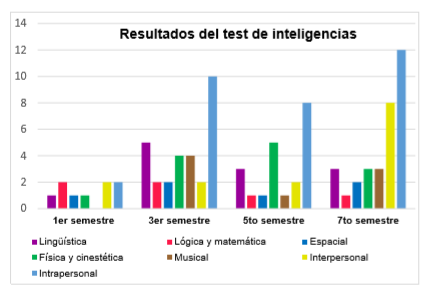
\includegraphics[width=1.0\textwidth]{./Imagenes/33}
	\caption{Es diseño de registro de los alumnos}
\end{figure}

\noindent \\

 \begin{figure}[H]
	\centering
	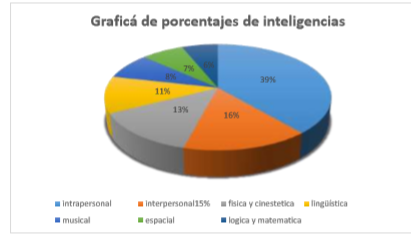
\includegraphics[width=1.0\textwidth]{./Imagenes/34}
	\caption{Es diseño de registro de los alumnos}
\end{figure}


\subsection{Prototipo}

 \begin{figure}[H]
	\centering
	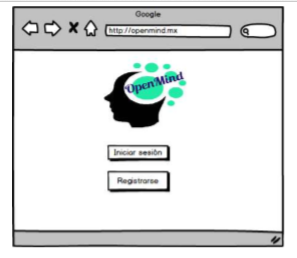
\includegraphics[width=1.0\textwidth]{./Imagenes/35}
	\caption{Es diseño de registro de los alumnos}
\end{figure}

 \begin{figure}[H]
	\centering
	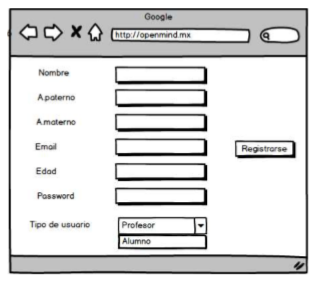
\includegraphics[width=1.0\textwidth]{./Imagenes/36}
	\caption{Es diseño de registro de los alumnos}
\end{figure}

 \begin{figure}[H]
	\centering
	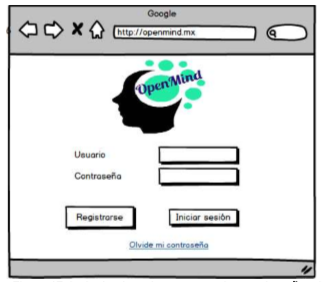
\includegraphics[width=1.0\textwidth]{./Imagenes/37}
	\caption{Es diseño de registro de los alumnos}
\end{figure}

 \begin{figure}[H]
	\centering
	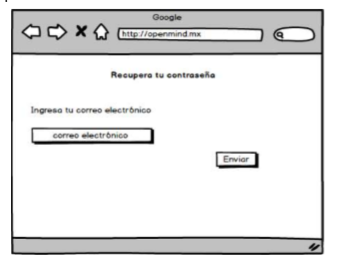
\includegraphics[width=1.0\textwidth]{./Imagenes/38}
	\caption{Es diseño de registro de los alumnos}
\end{figure}

 \begin{figure}[H]
	\centering
	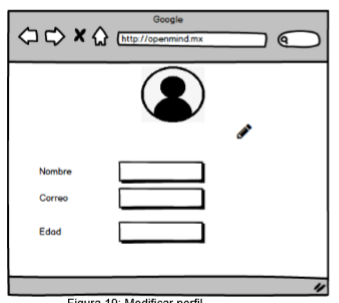
\includegraphics[width=1.0\textwidth]{./Imagenes/39}
	\caption{Es diseño de registro de los alumnos}
\end{figure}

 \begin{figure}[H]
	\centering
	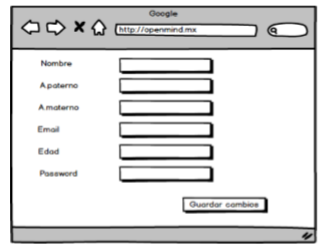
\includegraphics[width=1.0\textwidth]{./Imagenes/40}
	\caption{Es diseño de registro de los alumnos}
\end{figure}

 \begin{figure}[H]
	\centering
	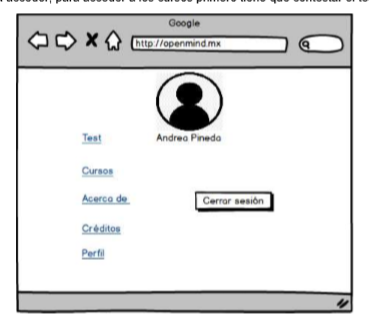
\includegraphics[width=1.0\textwidth]{./Imagenes/41}
	\caption{Es diseño de registro de los alumnos}
\end{figure}

 \begin{figure}[H]
	\centering
	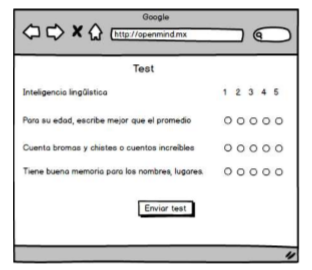
\includegraphics[width=1.0\textwidth]{./Imagenes/42}
	\caption{Es diseño de registro de los alumnos}
\end{figure}

 \begin{figure}[H]
	\centering
	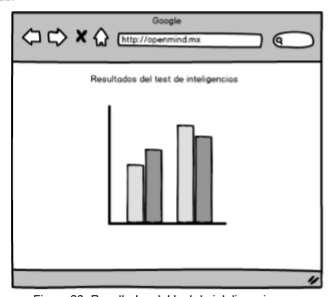
\includegraphics[width=1.0\textwidth]{./Imagenes/43}
	\caption{Es diseño de registro de los alumnos}
\end{figure}

 \begin{figure}[H]
	\centering
	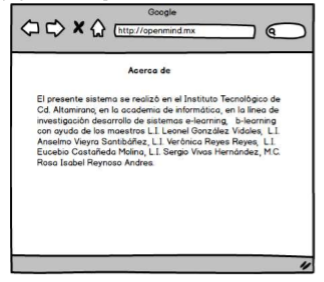
\includegraphics[width=1.0\textwidth]{./Imagenes/44}
	\caption{Es diseño de registro de los alumnos}
\end{figure}
% CONCLUSIONES 

% Las conclusiones deben ser redactadas con claridad y precisión ya que en ellas se presenta, el análisis de los resultados para comprobar los objetivos planteados, la justificación del proyecto, los alcances o limitaciones, la relación entre los resultados obtenidos, aportaciones logradas, deducciones obtenidas de la comparación y/o relación entre la teoría y la práctica. 

% Por lo tanto una conclusión consta de proposiciones inferidas de los resultados del trabajo, haciéndolas en forma deductiva, inductiva o análoga. Es importante mencionar que una conclusión es valida cuando proviene de un análisis objetivo de los resultados obtenidos haciendo resaltar las relaciones significativas. 

% Desde otro punto de vista se puede decir que las conclusiones son la síntesis de los logros obtenidos, de cada parte realizada en el proyecto de residencia profesional. 

% Para ayudar analizar o interpretar resultados obtenidos y en consecuencia formular conclusiones, se hace necesario seguir algunos puntos: 

% a) Exponer relaciones y generalizaciones que indiquen los resultados. 
% b) Señalar las excepciones, los aspectos no resueltos, las limitaciones. Evitar ocultar o alternar aquellos datos que no encajan bien. 
% c) Mostrar la concordancia o no concordancia con la justificación, los objetivos del proyecto o las metas planteadas, con otros proyectos, artículos, teorías, etc. 
% d) Describir las consecuencias teóricas del proyecto y sus posible aplicaciones prácticas. 


% RECOMENDACIONES 

% Esta sección corresponde a la descripción de las acciones ya sean inmediatas o mediatas que el residente debe proponer para el mejoramiento de un proceso, producto equipo, sistema de información, etc., en la empresa u organismo donde realizó la residencia profesional. 

% En otros términos, el residente expone con toda claridad las implicaciones prácticas de sus hallazgos, con el fin de plantear observaciones, actividades futuras, sugerencias, nuevos proyectos, etc., que redunden en el mejoramiento de la situación actual. 

% En todo planteamiento de una recomendación debe establecerse su justificación. Esto es, considerar el por qué y el para qué esas sugerencias, propuestas, actividades, planes de acción futuros o inmediatos. 

\chapter{Conclusiones y recomendaciones}\label{cap.conclusiones}
\section{Conclusiones}
\noindent Lorem ipsum dolor sit amet, consectetur adipiscing elit. Proin ullamcorper, sapien sed mattis commodo, lectus magna aliquet augue, consequat commodo nibh quam quis ante. Fusce et elit ac dui ultrices ultricies. Curabitur ultrices aliquam tempus. In iaculis turpis malesuada pellentesque lacinia. Proin ultrices lectus at augue ultrices scelerisque. Quisque ut sem est. Proin laoreet, purus eu vulputate fringilla, elit arcu condimentum dui, ut dapibus nunc est sit amet odio. Quisque ac est odio. Suspendisse non sagittis purus. Vestibulum a ullamcorper urna, aliquam pulvinar quam. Nullam dictum dolor dictum, pellentesque magna vel, ornare enim. Sed egestas, nisi non suscipit bibendum, enim erat ullamcorper felis, non pellentesque enim sem at ante. \\

\section{Recomendaciones}
\noindent Pellentesque imperdiet a tortor quis pharetra. Vivamus sit amet finibus ipsum. Ut commodo mauris non lacus semper consequat. Duis placerat a neque vel ultricies. Interdum et malesuada fames ac ante ipsum primis in faucibus. Aliquam lacus sem, vulputate vel sagittis et, auctor ac justo. Proin feugiat magna vitae sagittis interdum. Quisque suscipit euismod urna vitae vestibulum. Donec tincidunt ornare justo, ac sollicitudin metus elementum sit amet. Ut vitae laoreet magna. Etiam ut ex semper, eleifend lorem ut, sodales mi. Praesent non lobortis justo. Fusce ornare scelerisque ex a tempor. Phasellus maximus mauris eu magna rhoncus imperdiet. Duis dignissim auctor ipsum ut rhoncus. \\



\cleardoublepage
\addcontentsline{toc}{chapter}{Referencias}
\bibliographystyle{apalike3} % estilo de la bibliografía.
\bibliography{biblio}
\end{document}}